\documentclass[../main.tex]{subfiles}
\begin{document}

\chapter{Subspaces}
\label{chap:chap_3}

\emph{You should be familiar with}
	\begin{itemize}[noitemsep]
	\item Vector operations
	\item Row reducing a matrix
	\item Solving linear systems using row elimination
	\end{itemize}

\section[Introduction]{INTRODUCTION}
Throughout this chapter, we will be studying $\mathsf{R^{n}}$, the set of $n$-dimensional column vectors with real-valued components. We continue our study of matrices by considering a class of subsets of $\mathsf{R^{n}}$ called subspaces. These arise naturally, for example, when we solve a system of $n$ linear homogeneous equations in $n$ unknowns. The \emph{row space}, \emph{column space}, and \emph{null space} of the coefficient matrix play a role in many applications. We also study the concept of linear independence of a set of vectors,
which gives rise to the concept of subspace dimension.

\begin{remark}
	We will use the mathematical symbol $\in$ that means “contained in.” For instance, $u \in  \mathsf{R^2}$ means that $u$ is a vector in the plane, so $u = \begin{bmatrix}u_1\\ u_2 \end{bmatrix}$, where $u_1$, $u_2$ are real numbers.
\end{remark}

\section[Subspaces of \texttt{R}$^n$]{SUBSPACES OF $\texttt{R}^\mathbf{n}$}

\begin{definition}
	\label{defn:defn_3_1}
	A subset $S$ of $\mathsf{R^n}$ is called a subspace of $\mathsf{R^n}$ if

\begin{enumerate}[label=\textbf{\arabic*. }, noitemsep]
	\item The zero vector belongs to $S$ (i.e., $0 \in S$);
	\item If $u \in S$ and $v \in S$, then $u + v \in S$ ($S$ is said to be closed under vector addition);
	\item If $u \in S$ and $t \in R$, then $t u \in S$ ($S$ is said to be closed under scalar multiplication).
\end{enumerate}

$\mathsf{R^n}$ n is a subspace of itself, and we call $\mathsf{R^n}$ a \emph{vector space}. The complete definition of a vector space is very general, and
we will not provide it here. In \autoref{chap:chap_12}, we will introduce Fourier series as an example of a vector space whose elements are functions
\end{definition}

\begin{example} Let $A$ be an $n \times n$ matrix. Then the set of vectors $x \in Rn$ satisfying $A x = 0$ is a subspace of $\mathsf{R^n}$ called the \emph{null space} of $A$ and is denoted by N(A).\\
Verify each property of a subspace.
\begin{enumerate}[label=\textbf{\arabic*. }, noitemsep]
	 \item $A \times 0 = 0$, so $0 \times N(A)$.
	\item  If $x, y \in N(A)$, then $A x = 0$ and $A y = 0$, so $A(x + y) = Ax + Ay= 0 + 0 = 0$ and $x + y \in N(A).$
	\item If $x \in N(A)$ and $t \in R$, then $A(tx) = t(Ax) = t0 = 0$, so $tx \in N(A).$
\end{enumerate}
\end{example}

\begin{example} If $A =\begin{bmatrix} 1& 0\\ 0&1\end{bmatrix}$, the only solution to $Ax = 0$ is $x = 0$, so $N(A) = {0}$, the set consisting of just the zero vector.

The matrix $A =\begin{bmatrix} 1& 2\\ 2&4\end{bmatrix}$
row reduces to $\begin{bmatrix} 1& 2\\ 0 & 0 \end{bmatrix}$, so $x_1 +2x_2 = 0$,
and $x_1 = -2x_2$. $N(A)$ is the set of all scalar multiples of  $\begin{bmatrix} -2\\ 1 \end{bmatrix}$, a line in the plane.
\end{example}

\begin{figure}
	\centering
	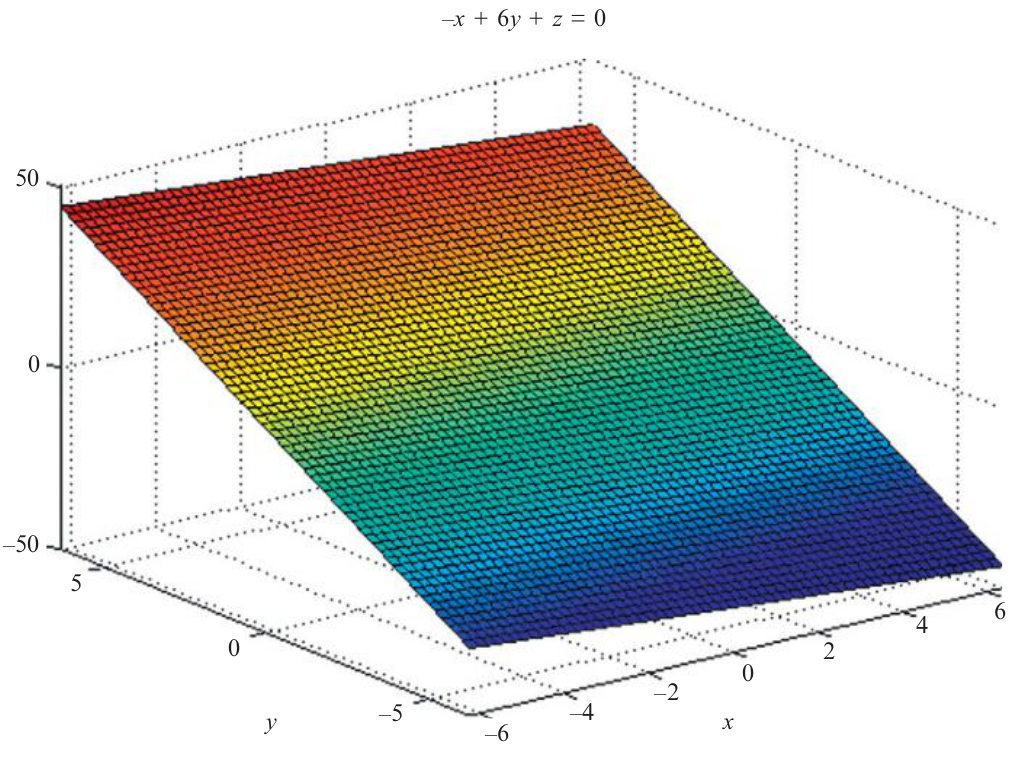
\includegraphics[width=0.7\linewidth]{fig_3_1}
	\caption{Subspace spanned by two vectors.}
	\label{fig:fig_3_1}
\end{figure}

In the vector space $\mathsf{R^3}$, take the vectors $\begin{Bmatrix} 1 & 1 & 5 \end{Bmatrix}^{T}$ and $\begin{Bmatrix} 2 & -1 & -8 \end{Bmatrix}^{T}$
and form all possible linear combinations
$c_{1}\begin{Bmatrix} 1 & 1 & 5 \end{Bmatrix}^{T} + c_{2} \begin{Bmatrix} 2 & -1 & -8 \end{Bmatrix}^{T}$. This set of vectors is a plane in $\mathsf{R^3}$ (\autoref{fig:fig_3_1}).

\begin{definition}
	\label{defn:defn_3_2}
	If $x_1, \ldots, x_m$ is a set of vectors in $\mathsf{R^n}$, then an expression of the form $c_1 x_1 + \ldots + c_m x_m$ is said to be a \emph{linear combination} of $x_1, \ldots ,x_m$.
\end{definition}

\begin{theorem}
	\label{theo:theo_3_1}
	Let $x_1, \ldots ,x_m \in \mathsf{R^n}$. Then the set consisting of all linear combinations

	$$c_1 x_1 + \ldots + c_m x_m,$$
	where $c_1, \ldots, c_m \in  R$ is a subspace of $\mathsf{R^n}$. This subspace is called the subspace spanned by $x_1,\ldots  ,x_m$ and is denoted by
	$$span~\{x_1, \ldots ,x_m\}.$$
\end{theorem}

\begin{proof}
	To show that the set of all linear combinations of $x_1, x_2,\ldots , x_m$ is a subspace, we must verify properties 1, 2, and 3 of  \autoref{defn:defn_3_1}.

	Property 1: $0 = 0 x_1 + \ldots +0 x_m$, so $0 \in span \{x_1, \ldots , x_m\}.$

	Property 2: If $x, y \in span \{x_1, \ldots ,x_m\}$, then $x = c_1 x_1 + \ldots + c_m x_m$ and $y = d_1 x_1 +\ldots + d_m x_m$, so
	$$x + y = (c_1 x_1 + \ldots + c_m x) + (d_1 x_1 + \ldots + d_m x_m)
	= (c_1 + d_1)x_1 + \ldots + (c_m + d_m) x_n$$
	and $x + y \in span \{x1, ... ,xm\}.$

	Property 3: If $x \in span \{x_1, \ldots  ,x_m\} and t \in \mathsf{R^n}$, then $x = c_1 x_1 + \ldots + c_m x_m, t_x = t(c_1 x_1 +\ldots + c_m x_m) = (tc_1) x_1 +\ldots + (tc_m) x_m \in span \{x1, \ldots  ,x_m\}.$
\end{proof}

\begin{definition}
	\label{defn:defn_3_3}
	If $A$ is an $n \times  n$ matrix, the subspace spanned by the columns of $A$ is a subspace of $\mathsf{R^n}$, called the \emph{column space} of $A$. Also, the subspace spanned by the rows of $A$ is a subspace of $\mathsf{R^n}$ called the \emph{row space} of $A$.
\end{definition}

\begin{example}  The $n \times  n$ identity matrix has columns
$$e_1 = \begin{Bmatrix} 1 & 0 & \ldots & 0 \end{Bmatrix}^{T}, e_2 = \begin{Bmatrix} 0 & 1 & \ldots & 0 \end{Bmatrix}^{T}, \ldots, e_{n-1} = \begin{Bmatrix} 0 & \ldots &1 & 0 \end{Bmatrix}^{T},  \begin{Bmatrix} 0 & \ldots & 0 & 1 \end{Bmatrix}^{T}. $$


Since $\left[\begin{array}{lllll}x_{1} & x_{2} & \ldots & x_{n-1} & x_{n}\end{array}\right]^{\mathrm{T}}=x_{1} e_{1}+x_{2} e_{2}+\cdots+x_{n-1} e_{n-1}+x_{n} e_{n}$, the column space of $I$ is $\mathsf{R}^{n} .$ The $e_{i}$ are called the
\emph{standard basis vectors}. Any vector in $\mathsf{R}^{n}$ can be written as a linear combination of the standard basis vectors. In a similar fashion, the rows of I span $\mathsf{R}^{n}$.
\end{example}

\begin{example} The equation $2 x-3 y+5 z=0$ defines a relationship between the components of a vector $\left[\begin{array}{lll}x & y & z\end{array}\right]^{\mathrm{T}}$. Find the subspace $S$ of $\texttt{R}^{3}$ spanned by all such vectors. If $[x, y, z]^{\mathrm{T}} \in S$, then $x=\frac{3}{2} y-\frac{5}{2} z$, so
$$
\left[\begin{array}{l}
x \\
y \\
z
\end{array}\right]=\left[\begin{array}{l}
\frac{3}{2} y-\frac{5}{2} z \\
y \\
z
\end{array}\right]=y\left[\begin{array}{l}
\frac{3}{2} \\
1 \\
0
\end{array}\right]+z\left[\begin{array}{l}
-\frac{5}{2} \\
0 \\
1
\end{array}\right].
$$
Thus, $S$ is the subspace spanned by $\left[\begin{array}{l}\frac{3}{2} \\ 1 \\ 0\end{array}\right]$ and $\left[\begin{array}{l}-\frac{5}{2} \\ 0 \\ 1\end{array}\right] .$ This subspace is not $\mathsf{R}^{3}$. Consider the vector $\left[ \begin{array}{l}1 \\ 2 \\ 3\end{array}\right]$ and determine if it can be written as a linear combination of $\left[\begin{array}{l}\frac{3}{2} \\ 1 \\ 0\end{array}\right]$ and $\left[\begin{array}{l}-\frac{5}{2} \\ 0 \\ 1\end{array}\right] .$ There must be scalars $c_{1}$ and $c_{2}$ such that
$$
c_{1}\left[\begin{array}{l}
\frac{3}{2} \\
1 \\
0
\end{array}\right]+c_{2}\left[\begin{array}{l}
-\frac{5}{2} \\
0 \\
1
\end{array}\right]=\left[\begin{array}{l}
1 \\
2 \\
3
\end{array}\right]
$$
This requires that
$$
\frac{3}{2} c_{1}-\frac{5}{2} c_{2}=1
$$
We must have $c_{1}=2$ and $c_{2}=3$, but
$$
\frac{3}{2}(2)-\frac{5}{2}(3)=-4 \frac{1}{2} \neq 1 .
$$
The two vectors do not span $\texttt{R}^{3}$. In general, it takes $n$ vectors to span $\texttt{R}^{n}$
\end{example}

\section[Linear Independence]{LINEAR INDEPENDENCE}

\begin{definition}
	\label{defn:defn_3_4}The concept of linear independence of a set of vectors in $\mathsf{R}^{n}$ is extremely important in linear algebra and its applications.

Vectors $x_{1}, \ldots, x_{m}$ in $\mathsf{R}^{n}$ are said to be \emph{linearly dependent} if there exist scalars $c_{1}, \ldots, c_{m}$, \emph{not all zero}, such that
\begin{equation}
\label{eq:eq_3_1}
c_{1} x_{1}+\cdots+c_{m} x_{m}=0 .
\end{equation}

Suppose $c_{i} \neq 0 .$ Then, $x_{i}=-\left(c_{1} x_{1}+c_{2} x_{2}+\cdots+c_{i-1} x_{i-1}+c_{i+1} x_{i+1}+\cdots+c_{m} x_{m}\right) / c_{i} .$ The vector $x_{i}$ can be written as a linear combination of the remaining vectors; in other words, it is dependent on them. The vectors $x_{1}, \ldots, x_{m}$ are called \emph{linearly independent} if they are not linearly dependent. To test for linear independence, \autoref{eq:eq_3_1} is a linear homogeneous equation with unknowns $\left[\begin{array}{lllll}c_{1} & c_{2} & \ldots & c_{m-1} & c_{m}\end{array}\right]^{\mathrm{T}}$. The vectors are linearly independent if the system has only the trivial solution $c_{1}=0, \ldots, c_{m}=0 .$ Conversely, if $x_{1}, x_{2}, \ldots, x_{m}$ are linearly independent, then the homogeneous system has only the trivial solution.
\end{definition}

\begin{example} Are the following three vectors in $\mathsf{R}^{3}$ linearly independent or dependent?
$$
x_{1}=\left[\begin{array}{l}
1 \\
2 \\
3
\end{array}\right], \quad x_{2}=\left[\begin{array}{c}
-1 \\
1 \\
2
\end{array}\right], \quad x_{3}=\left[\begin{array}{c}
-1 \\
7 \\
12
\end{array}\right]
$$
Form
$$
c_{1}\left[\begin{array}{l}
1 \\
2 \\
3
\end{array}\right]+c_{2}\left[\begin{array}{c}
-1 \\
1 \\
2
\end{array}\right]+c_{3}\left[\begin{array}{c}
-1 \\
7 \\
12
\end{array}\right]=\left[\begin{array}{l}
0 \\
0 \\
0
\end{array}\right]
$$

This corresponds to the homogeneous system.
$$
\begin{gathered}
{\left[\begin{array}{ccc}
	1 & -1 & -1 \\
	2 & 1 & 7 \\
	3 & 2 & 12
	\end{array}\right]\left[\begin{array}{l}
	c_{1} \\
	c_{2} \\
	c_{3}
	\end{array}\right]=0} \\
{\left[\begin{array}{ccc}
	1 & -1 & -1 \\
	2 & 1 & 7 \\
	3 & 2 & 12
	\end{array}\right] \begin{array}{l}
	\overrightarrow{R 2=R 2-2 R 1} \\ R 3=R 3-3 R 1
	\end{array}\left[\begin{array}{ccc}
	1 & -1 & -1 \\
	0 & 3 & 9 \\
	0 & 5 & 15
	\end{array}\right] \overrightarrow{R 3=R 3-(5 / 3) R 2}\left[\begin{array}{ccc}
	1 & -1 & -1 \\
	0 & 3 & 9 \\
	0 & 0 & 0
	\end{array}\right] .}
\end{gathered}
$$
The row of zeros in the row-reduced matrix indicates that there are infinitely many solutions to the homogeneous system, so $x_{1}, x_{2}, x_{3}$ are linearly dependent.
\end{example}

\begin{example}  Are the vectors
\label{exm:exm_3_6}
$u =\left[\begin{array}{c}1\\2\\-1\end{array}\right],
v =\left[\begin{array}{c}1\\-1\\3\end{array}\right],
w =\left[\begin{array}{c}1\\2\\3\end{array}\right], $
linearly independent? Let $c_1 u + c_2 v + c_3 w = 0.$ This corresponds to the linear homogeneous system
$$
\begin{gathered}
{\left[\begin{array}{ccc}
	1 & 1 & 1 \\
	2 & -1 & 2 \\
	-1 & 3 & 3
	\end{array}\right]\left[\begin{array}{l}
	c_{1} \\
	c_{2} \\
	c_{3}
	\end{array}\right]=0 .} \\
{\left[\begin{array}{ccc}
	1 & 1 & 1 \\
	2 & -1 & 2 \\
	-1 & 3 & 3
	\end{array}\right] \begin{array}{c}
	\overrightarrow{R 2=R 2-2 R 1} \\
	R 3=R 3-(-1) R 1
	\end{array}\left[\begin{array}{ccc}
	1 & 1 & 1 \\
	0 & -3 & 0 \\
	0 & 4 & 4
	\end{array}\right] \overrightarrow{R 3=R 3-(-4 / 3) R 2}\left[\begin{array}{ccc}
	1 & 1 & 1 \\
	0 & -3 & 0 \\
	0 & 0 & 4
	\end{array}\right]}
\end{gathered}
$$
The final system in the row-elimination process has the unique solution $c_{1}=c_{2}=c_{3}=0$, so $u, v$, and $w$ are linearly independent.
\end{example}

\section[Basis of the Subspace]{BASIS OF A SUBSPACE}
We now come to the fundamental concept of a \emph{basis} for a subspace.

\begin{definition}
	\label{defn:defn_3_5}Vectors $x_{1}, \ldots, x_{m}$ belonging to a subspace $S$ are said to form a basis for $S$ if
\begin{enumerate}[label=\textbf{\arabic*. }, noitemsep]
	\item $x_{1}, \ldots, x_{m}$ span $S$.
	\item$x_{1}, \ldots, x_{m}$ are linearly independent.
\end{enumerate}
\end{definition}

\begin{example} The standard basis vectors $e_{1}, \ldots, e_{n}$ form a basis for $\mathsf{R}^{n} .$ This is the reason for the term "standard basis." If $x=\left[\begin{array}{c}x_{1} \\ \vdots \\ x_{n}\end{array}\right]$, then $x=x_{1} e_{1}+x_{2} e_{2}+\cdots+x_{n} e_{n}$, so $e_{1}, e_{2}, \ldots, e_{n}$ span $R^{n} .$ They are linearly independent, since if
$c_{1} e_{1}+c_{2} e_{2}+\cdots+c_{n} e_{n}=\left[\begin{array}{c}c_{1} \\ c_{2} \\ \vdots \\ c_{n}\end{array}\right]=0$, then $c_{1}=c_{2}=\cdots=c_{n}=0$
\end{example}

A subspace normally has more than one basis; for instance, let $u, v$, and $w$ be the linearly independent vectors of \autoref{exm:exm_3_6}.  To show that the vectors are a basis for $\mathsf{R}^{3}$, it is necessary to show that the vectors span  $\mathsf{R}^{3} .$ Let $x$ be any vector in $\mathsf{R}^{3}$. There must be a linear combination of $u, v$, and $w$ that equals $x ;$ in other words, there must be scalars $c_{1}, c_{2}, c_{3}$, such that $c_{1} u+c_{2} v+c_{3} w=x .$ This is a system of linear equations
$$
\left[\begin{array}{ccc}
1 & 1 & 1 \\
2 & -1 & 2 \\
-1 & 3 & 3
\end{array}\right]\left[\begin{array}{l}
c_{1} \\
c_{2} \\
c_{3}
\end{array}\right]=\left[\begin{array}{l}
x_{1} \\
x_{2} \\
x_{3}
\end{array}\right].
$$



Form the augmented matrix
$\left[\begin{array}{ccc|c}
1 & 1 & 1 & x_{1}\\
2 & -1 & 2 & x_{2}\\
-1 & 3 & 3 & x_{3}\\
\end{array}\right]$. The row-reduction operations performed in Example 3.6 show that there is a unique solution for
$\left[\begin{array}{c}
c_{1}\\
c_{2}\\
c_{3}
\end{array}\right]$, and so $u, v$, and $w$ form a basis for $\mathsf{R}^{3}$.

There are some important properties of a basis that are stated in  \autoref{theo:theo_3_2}

\begin{theorem}
	\label{theo:theo_3_2}
	If $S$ is a subspace of $\mathsf{R}^{n}$, then

	\begin{enumerate}[label=\textbf{\arabic*. }, noitemsep]
	\item Each vector in a basis for $S$ must be nonzero.
	\item If $u$ is a vector in $S$, there is one and only one way to write $u$ as a linear combination of basis vectors for $S$.
	\item A subspace span $\{x_1, \ldots ,x_m\}$, where at least one of $x_1, \ldots ,x_m$ is nonzero, has a basis $v_1, \ldots ,v_p,$ where $p \leq m.$
	\end{enumerate}
\end{theorem}

\begin{proof}
	To prove 1, assume that $x_1, \ldots ,x_m$ is a basis for $S$, and that $x_1 = 0$. Then we have the nontrivial linear combination 1 $(x_1) + 0 (x_2) +\ldots + 0 (x_m) = 0$, and $x_1, \ldots ,x_m$ are linearly dependent.

	Let $x_1, \ldots ,x_m$ be a basis for $S$. Assume that $u = c_1 x_1 + c_2 x_2 + \ldots + c_m x_m$ and that $u = d_1 x_1 + d_2 x_2 +\ldots + d_m x_m$. Subtract the two equations to obtain
	$$(c_1 - d_1) x_1 + (c_2 - d_2) x_2 +\ldots + (c_m - d_m) x_m = 0.$$
	Since $x_1, \ldots ,x_m$ are linearly independent, $(c_1 - d_1) = 0, (c_2 - d_2) = 0, \ldots ,(c_m - d_m) = 0$, and $c_i = d_i, 1 \leq i \leq m.$ We have proved 2.

	Statement 3 tells us that the span of any set of vectors has a basis as long as all the vectors are not zero. Scan $x_1, \ldots ,x_m$ from left to right and let $x_{j_1}$ be the first nonzero vector. If $j_1 = m$ or all the vectors $x_k, j_1 + 1 \leq k \leq m$ are multiples of $x_{j_1}$ , then $p = 1$. Otherwise, let $x_{j_2}$ be the next nonzero vector following $x_{j_1}$ such that $x_{j_2}$ is not a multiple of $x_{j_1}$ . If $j_2 = m$ or if all the vectors $x_k, j_2 + 1 \leq k \leq m$ are linear combinations of $x_{j_1}$ and $x_{j_2}$ , then $p = 2$. This argument will eventually terminate with a set of vectors $x_{j_1} , x_{j_2} , \ldots  , x_{j_p}$  that must be linearly independent. Any vectors among $x_1, \ldots ,x_m$ that were combinations of other vectors have been eliminated, so $x_{j_1} , x_{j_2} , \ldots  , x_{j_p}$ spans $S$, and is a basis for $S$.
\end{proof}

\begin{example} Let $x$ and $y$ be linearly independent vectors in $\mathsf{R}^{n}$. Consider the subspace span $\{0, 2x, x, -y, x + y\}$. Apply the technique used in proving part 3 of \autoref{theo:theo_3_1} Skip over 0 and record $2x$ as a nonzero vector. Move right and discard $x$ because it is a multiple of $2\times$. The next vector, $-y$, is not a multiple of $x$ because $x$ and $y$ are linearly independent. The final vector $x + y$ is a linear combination of $2x$ and $-y$. The subspace $\{0, 2x, x, -y, x + y\}$ has a basis $2x, -y.$
\end{example}

By using arguments similar to those in \autoref{theo:theo_3_2}, the following claims can be proved. The proofs will not be provided, but the interested reader can consult Strang \cite[pp. 175-175]{ref8} for very readable arguments.

\emph{Claim 3.1}. If $S$ is a subspace of  $\mathsf{R}^{n}$, then
\begin{enumerate}[label=\textbf{\arabic*}), noitemsep]
	\item Any two bases for a subspace $S$ must contain the same number of elements. This number is called the dimension of $S$ and is written dim $S$.
	\item If a subspace has dimension $m$, then any set of $m$ linearly independent vectors is a basis for $S$.
\end{enumerate}

\section[The Rank of a Matrix]{THE RANK OF A MATRIX}
In this section, we will determine how to find a basis for the row space of a matrix and discuss the relationship between the row space and the column space of a matrix.

\begin{definition}
	\label{defn:defn_3_6}
	 The number of elements in a basis for the row space is called the \emph{rank} of the matrix.
\end{definition}

The rank is defined for any $m \times n$ matrix, but we will deal only with square matrices for now. The process we develop to find the rank of a matrix will involve row reductions, but we will go beyond just getting to upper-triangular form and will also “zero out” as many elements in the upper triangle as we can. The process is illustrated with examples and is based upon the following lemma and a theorem that follows from it.



\begin{lemma}
	\label{lem:lem_3_1}
	Subspaces span $\left\{x_{1}, x_{2}, \ldots, x_{r}\right\}$ and $\operatorname{span}\left\{y_{1}, y_{2}, \ldots, y_{s}\right\}$ are equal if each of $x_{1}, x_{2}, \ldots, x_{r}$ is a linear combination of $y_{1}, y_{2}, \ldots, y_{s}$ and each of $y_{1}, y_{2}, \ldots, y_{s}$ is a linear combination of $x_{1}, x_{2}, \ldots, x_{r}$.
\end{lemma}

\begin{proof}
	Let $x=c_{1} x_{1}+\ldots+c_{r} .$ Since each of $x_{1}, x_{2}, \ldots, x_{r}$ is a linear combination of $y_{1}, y_{2}, \ldots, y_{s}$, it follows that $x$ is a linear combination of $y_{1}, y_{2}, \ldots, y_{s} .$ Similarly, if $y=d_{1} y_{1}+\cdots+d_{s} y_{s}$, then $y$ is a linear combination of $x_{1}, x_{2}, \ldots, x_{r .}$ This shows the two subspaces are equal.
\end{proof}

\begin{theorem}
	\label{theo:theo_3_3}
	The row space of a matrix is the same as the row space of any matrix derived from it using row reduction.
\end{theorem}

\begin{proof}
	Suppose that matrix $B$ is obtained from matrix $A$ by a sequence of elementary row operations. Then each row of $B$ is a linear combination of the rows of $A$. But $A$ can be obtained from $B$ by a sequence of elementary row operations, so each row of $A$ is a linear combination of the rows of $B$. By \autoref{lem:lem_3_1}, the two row spaces are equal.
\end{proof}

\begin{example}  $A=\left[\begin{array}{ll}1 & 2 \\ 2 & 4\end{array}\right]$. The upper-triangular form for $A$ is $B=\left[\begin{array}{cc}1 & 2 \\ 0 & 0\end{array}\right]$, and we cannot eliminate any more elements. The row space of $A$ and $B$ is the same and consists of all multiples of the vector
$\left[\begin{array}{cc} 1 & 2\end{array}\right].$
Hence,
 $\left[\begin{array}{cc} 1 & 2\end{array}\right]$
 is a basis for the row space of $A$ and the rank of $A$ is 1.

 Find the row space and rank of $A=\left[\begin{array}{ll}1 & 2 \\ 3 & 4\end{array}\right]$. We begin row reduction with
$$
\left[\begin{array}{ll}
1 & 2 \\
3 & 4
\end{array}\right] \overrightarrow{R 2=R 2-3 R 1}\left[\begin{array}{cc}
1 & 2 \\
0 & -2
\end{array}\right]
$$
Continue on and use the $-2$ in row $2$, column $2$ to eliminate the element above it in row $1$ , column $2 .$ Also, remember we can multiply any row by a constant during row reduction.
$$
\left[\begin{array}{cc}
1 & 2 \\
0 & -2
\end{array}\right] \overrightarrow{R 1=R 1-(-1) R 2}\left[\begin{array}{cc}
1 & 0 \\
0 & -2
\end{array}\right] \overrightarrow{R 2=R 2 /(-2)}\left[\begin{array}{ll}
1 & 0 \\
0 & 1
\end{array}\right]
$$
The row space consists of all linear combinations of the vectors $[10]$ and $[0 \quad 1]$, and so the row space is $\mathsf{R}^{2}$, and the rank of $A$ is 2.
\end{example}

\begin{example}  Consider $A = \left[\begin{array}{ccc}
1 & 0 & 2 \\
0 & 1 & 3 \\
1 & 4 & 5
\end{array}\right]
$. Perform row reductions to determine a basis for the row space and the
rank of A.
$$
\left[\begin{array}{lll}
1 & 0 & 2 \\
0 & 1 & 3 \\
1 & 4 & 5
\end{array}\right] \overline{R 3=R 3-(1) R 1}\left[\begin{array}{lll}
1 & 0 & 2 \\
0 & 1 & 3 \\
0 & 4 & 3
\end{array}\right] \overrightarrow{R 3=R 3-4 R 2}\left[\begin{array}{llc}
1 & 0 & 2 \\
0 & 1 & 3 \\
0 & 0 & -9
\end{array}\right]
$$
This is upper-triangular form, but continue eliminating as many elements as we can. To make things easier, divide row $3$ by $-9$
$$
\left[\begin{array}{ccc}
1 & 0 & 2 \\
0 & 1 & 3 \\
0 & 0 & -9
\end{array}\right] \overrightarrow{R 3=R 3 /(-9)}\left[\begin{array}{lll}
1 & 0 & 2 \\
0 & 1 & 3 \\
0 & 0 & 1
\end{array}\right] \begin{array}{c}
\overrightarrow{R 2=R 2-3 R 3} \\ R 1=R 1-2 R 3
\end{array}\left[\begin{array}{lll}
1 & 0 & 0 \\
0 & 1 & 0 \\
0 & 0 & 1
\end{array}\right]
$$
The row space of $A$ is $\mathsf{R}^{3}$, and the rank of $A$ is 3 . Note that this matrix has no null space; in other words, the null space of $A$ is the empty set.
\end{example}

\begin{example}  Let $A=\left[\begin{array}{cccc}2 & 5 & -4 & 1 \\ 3 & 8 & -9 & 2 \\ 1 & 1 & 7 & -1 \\ 1 & 2 & 1 & 0\end{array}\right]$. Perform row reductions to determine a basis for the row space and the rank
of $A$
$$
\left[\begin{array}{cccc}
2 & 5 & -4 & 1 \\
3 & 8 & -9 & 2 \\
1 & 1 & 7 & -1 \\
1 & 2 & 1 & 0
\end{array}\right] \begin{aligned}
&\overrightarrow{R 2=R 2-(3 / 2) R 1} \\
&R 3=R 3-(1 / 2) R 1 \\
&R 4=R 4-(1 / 2) R 1
\end{aligned}\left[\begin{array}{cccc}
2 & 5 & -4 & 1 \\
0 & \frac{1}{2} & -3 & \frac{1}{2} \\
0 & -\frac{3}{2} & 9 & -\frac{3}{2} \\
0 & -\frac{1}{2} & 3 & -\frac{1}{2}
\end{array}\right] \begin{aligned}
&\overrightarrow{R 3=R 3-(-3) R 2} \\
&R 4=R 4-(-1) R 2
\end{aligned}\left[\begin{array}{cccc}
2 & 5 & -4 & 1 \\
0 & \frac{1}{2} & -3 & \frac{1}{2} \\
0 & 0 & 0 & 0 \\
0 & 0 & 0 & 0
\end{array}\right]
$$
Now eliminate the 5 in row 1, column 2 .
$$
\left[\begin{array}{cccc}
2 & 5 & -4 & 1 \\
0 & \frac{1}{2} & -3 & \frac{1}{2} \\
0 & 0 & 0 & 0 \\
0 & 0 & 0 & 0
\end{array}\right] \overrightarrow{R 1=R 1-(10) R 2}\left[\begin{array}{cccc}
2 & 0 & 26 & -4 \\
0 & \frac{1}{2} & -3 & \frac{1}{2} \\
0 & 0 & 0 & 0 \\
0 & 0 & 0 & 0
\end{array}\right] .
$$
We cannot go any further without removing the zero we just produced; however, let's multiply row 1 by $\frac{1}{2}$ and row 2 by 2 to make the leading element of each nonzero row 1 .
$$
\left[\begin{array}{cccc}
2 & 0 & 26 & -4 \\
0 & \frac{1}{2} & -3 & \frac{1}{2} \\
0 & 0 & 0 & 0 \\
0 & 0 & 0 & 0
\end{array}\right] \begin{gathered}
\overrightarrow{R 1=(1 / 2) R 1} \\
R 2=(2) R 2
\end{gathered}\left[\begin{array}{cccc}
1 & 0 & 13 & -2 \\
0 & 1 & -6 & 1 \\
0 & 0 & 0 & 0 \\
0 & 0 & 0 & 0
\end{array}\right]
$$
The rank of $A$ is 2 , and $\left[\begin{array}{llll}1 & 0 & 13 & -2\end{array}\right],\left[\begin{array}{llll}0 & 1 & -6 & 1\end{array}\right]$ are a basis for the row space.
\end{example}

This process of finding the rank of a matrix seems somewhat disorganized. In reality, the rank of a matrix is found by computing the singular value decomposition (SVD). We will discuss the SVD in \autoref{chap:chap_15}, and will show how to compute it accurately and efficiently in \autoref{chap:chap_23}.

\begin{example} \label{exm:exm_3_12}We have computed the row space for some matrices, and now we will find the null space and nullity of a matrix. Let $A$ be the matrix of Example $3.11 .$ The null space of $A$ is the subspace of vectors $x$ such that $A x=0 .$ Using the computations in Exercise $3.11$, we have
$$
A=\left[\begin{array}{cccc}
2 & 5 & -4 & 1 \\
3 & 8 & -9 & 2 \\
1 & 1 & 7 & -1 \\
1 & 2 & 1 & 0
\end{array}\right] \Longrightarrow\left[\begin{array}{cccc}
1 & 0 & 13 & -2 \\
0 & 1 & -6 & 1 \\
0 & 0 & 0 & 0 \\
0 & 0 & 0 & 0
\end{array}\right]
$$
This says that
$$
\begin{aligned}
x_{1}+13 x_{3}-2 x_{4} &=0, \\
x_{2}-6 x_{3}+x_{4} &=0.
\end{aligned}
$$
From these equations,
$x_{1}=-13 x_{3}+2 x_{4}, x_{2}=6 x_{3}-x_{4}$. The variables $x_{4}$ and $x_{3}$ are arbitrary, so a basis for the null space of $A$ is
$$
z_{1}=\left[\begin{array}{c}
-13 \\
6 \\
1 \\
0
\end{array}\right], \quad z_{2}=\left[\begin{array}{c}
2 \\
-1 \\
0 \\
1
\end{array}\right]
$$
Note the presence of two zero rows and a nullity of two.
\end{example}

Find the rank of a matrix using the MATLAB command \texttt{rank(A)}. The command \texttt{Z = null(A)} is used to find a basis for the null space of a matrix as a set of column vectors that form the matrix $Z$. If you only want the nullity of the matrix,
obtain the number of columns of the matrix returned by \texttt{null} using \texttt{size(null(A),2).}



\begin{example} \label{exm:exm_3_13} Note that in the MATLAB output, \texttt{( A*Z ( : ,1) )'} should be a row vector of zeros, but very small nonzero
vector components are the result. In \autoref{chap:chap_8}, we will discuss why this occurs.
\begin{lstlisting}[numbers=none,frame=none]
	>> A = [2 5 -4 1;3 8 -9 2;1 1 7 -1;1 2 1 0];
	>> rank(A)

	ans =
				2

	>> Z = null(A);
	>> ( A * Z( : ,1 ) )'

	ans =
		1.0e-014 *
			-0.0860	 -0.1277	 -0.0583	 -0.0472

	>> size(null(A),2)
	ans =
			2
\end{lstlisting}
\end{example}

Notice that in Example 3.13, the rank of the matrix is 2 and the nullity is 2, so rank + nullity = 4, the matrix size. This is an example of the relation between the dimension of the row space of a matrix and its null space.

\begin{theorem}
	\label{theo:theo_3_4}
	If $A$ is an $n \times n$ matrix, the rank of $A$ plus the nullity of $A$ equals $n$.
\end{theorem}
We will prove this result in Chapter 15 when we present the singular value decomposition of a matrix.

\begin{remark}
	An $n \times n$ matrix $A$ is said to have \emph{full rank} if the rank of $A$ is $n$. It follows from \autoref{theo:theo_3_4} that if a matrix has full rank, then there is no null space.
\end{remark}

\begin{example}\label{exm:exm_3_14}  Let $A$ be the matrix in Examples \ref{exm:exm_3_12} and \ref{exm:exm_3_13}. As stated in \autoref{defn:defn_3_1}, the column space of a matrix $A$ is the subspace spanned by the columns of $A$. We will find a basis for the column space of $A$, the subspace spanned by $\left[\begin{array}{l}2 \\ 3 \\ 1 \\ 1\end{array}\right],\left[\begin{array}{l}5 \\ 8 \\ 1 \\ 2\end{array}\right],\left[\begin{array}{c}-4 \\ -9 \\ 7 \\ 1\end{array}\right],\left[\begin{array}{c}1 \\ 2 \\ -1 \\ 0\end{array}\right] .$ Form $A^{\mathrm{T}}$, the matrix whose rows are the columns of $A$ and perform row operations on $A^{\mathrm{T}}$.
$$
\begin{aligned}
&{\left[\begin{array}{cccc}
	2 & 3 & 1 & 1 \\
	5 & 8 & 1 & 2 \\
	-4 & -9 & 7 & 1 \\
	1 & 2 & -1 & 0
\end{array}\right] \begin{array}{r}
	\overrightarrow{R 2=R 2-(5 / 2) R 1} \\
	R 3=R 3-(-2) R 1 \\
	R 4=R 4-(1 / 2) R 1
\end{array}\left[\begin{array}{cccc}
	2 & 3 & 1 & 1 \\
	0 & 1 / 2 & -3 / 2 & -1 / 2 \\
	0 & -3 & 9 & 3 \\
	0 & 1 / 2 & -3 / 2 & -1 / 2
	\end{array}\right]} \\
&\left[\begin{array}{cccc}
2 & 3 & 1 & 1 \\
0 & 1 / 2 & -3 / 2 & -1 / 2 \\
0 & -3 & 9 & 3 \\
0 & 1 / 2 & -3 / 2 & -1 / 2
\end{array}\right] \begin{array}{c}
\overrightarrow{R 3=R 3-(-6) R 2} \\
R 4=R 4-(1) R 2
\end{array}\left[\begin{array}{cccc}
2 & 3 & 1 & 1 \\
0 & 1 / 2 & -3 / 2 & -1 / 2 \\
0 & 0 & 0 & 0 \\
0 & 0 & 0 & 0
\end{array}\right] \\
&{\left[\begin{array}{cccc}
	2 & 3 & 1 & 1 \\
	0 & 1 / 2 & -3 / 2 & -1 / 2 \\
	0 & 0 & 0 & 0 \\
	0 & 0 & 0 & 0
	\end{array}\right]
	\overrightarrow{R 1=R 1-(6) R 2}
	\left[\begin{array}{cccc}
	2 & 0 & 10 & 4 \\
	0 & 1 / 2 & -3 / 2 & -1 / 2 \\
	0 & 0 & 0 & 0 \\
	0 & 0 & 0 & 0
	\end{array}\right]}
\end{aligned}
$$


This is as far as we can go, so a basis for the column space of $A$ is
$$
\left[\begin{array}{c}
2 \\
0 \\
10 \\
4
\end{array}\right],\left[\begin{array}{c}
0 \\
1 / 2 \\
-3 / 2 \\
-1 / 2
\end{array}\right]
$$
\end{example}
Notice that the dimension of the column space of $A$ in  \autoref{exm:exm_3_14} is the same as the dimension of the row space of
$A$. This is true for any $m \times n$ matrix, and we will prove this in \autoref{chap:chap_15}

\section[Chapter Summary]{CHAPTER SUMMARY}

\subsection*{Subspaces of $\mathsf{R}^{n}$}
$\mathsf{R}^{n}$ is a vector space, and subsets of $\mathsf{R}^{n}$, including $\mathsf{R}^{n}$ itself, are called subspaces. A subspace satisfies three properties:

\begin{itemize}[noitemsep]

\item The zero vector is in the subspace.

\item If $x$ is a vector in the subspace, then $c x$ is in the subspace, where $c$ is a number.

\item If $x$ and $y$ are in the subspace, then so is $x+y$.
\end{itemize}
If $x_{1}, x_{2}, \ldots, x_{k}$ are in $\mathsf{R}^{n}, k \leq n$, then the set of all linear combinations $c_{1} x_{1}+c_{2} x_{2}+\cdots+c_{k} x_{k}$ is a subspace, and is said to be the subspace, $S$, of $\mathsf{R}^{n}$ spanned by $x_{1}, \ldots, x_{k}$, and we write
$$S=\operatorname{span}\left\{x_{1}, \ldots, x_{k}\right\}$$

\subsection*{Linear Independence}
A collection of vectors is linearly independent if no vector can be written as a linear combination of the others. For instance. if $u=\left[\begin{array}{c}1 \\ 0 \\ -1\end{array}\right], v=\left[\begin{array}{l}2 \\ 7 \\ 3\end{array}\right], w=\left[\begin{array}{l}1 \\ 0 \\ 0\end{array}\right]$, then these vectors are linearly independent. But, if we let $v=\left[\begin{array}{c}4 \\ 0 \\ -1\end{array}\right]$, then
$v=u+3 w$, and the vectors are linearly dependent. In general, a set of vectors $v_{1}, \ldots, v_{k}$ is linearly independent if
$$
c_{1} v_{1}+c_{2} v_{2}+\cdots+c_{k} v_{k}=0
$$
only when $c_{1}=c_{2}=\cdots=c_{k}=0 .$ This means that the homogeneous system
$$
\left[\begin{array}{lllll}
v_{1} & v_{2} & \ldots & v_{k-1} & v_{k}
\end{array}\right]\left[\begin{array}{c}
c_{1} \\
c_{2} \\
\vdots \\
c_{k-1} \\
c_{k}
\end{array}\right]=0
$$
has only the zero solution.

\subsection*{Basis of a Subspace}
The basis for a subspace is a set of vectors that span the subspace and are linearly independent. For instance, the standard basis for $\mathsf{R}^{n}$ is
$$
e_{1}=\left[\begin{array}{llll}
1 & \ldots & 0 & 0
\end{array}\right]^{\mathrm{T}}, e_{2}=\left[\begin{array}{llll}
0 & 1 & \ldots & 0
\end{array}\right]^{\mathrm{T}}, \ldots, e_{n}=\left[\begin{array}{llll}
0 & \ldots & 0 & 1
\end{array}\right]^{\mathrm{T}}
$$



A subspace can have more than one basis. For instance, the vectors $u, v, w$ in Section “Linear Independence” are a basis for $\mathsf{R}^{3}$, as is $e_1, e_2, e_3$. However, all bases for a subspace have the same number of vectors, and this number is the dimension of the subspace.

\subsection*{Matrix Rank}
The rank of a matrix is the dimension of the subspace spanned by its rows. As we will prove in \autoref{chap:chap_15}, the dimension of the column space is equal to the rank. This has important consequences; for instance, if $A$ is an $m \times n$ matrix and $m \geq n$, then rank $(\mathrm{A}) \leq \mathrm{n}$, but if $m<n$, then rank $(\mathrm{A}) \leq \mathrm{m} .$ It follows that if a matrix is not square, either its columns or its rows must be linearly dependent.

For small square matrices, perform row elimination in order to obtain an upper-triangular matrix. If a row of zeros occurs, the rank of the matrix is less than $n$, and it is singular. As we will see in \textcolor{blue}{Chapters \ref{chap:chap_7}},\ref{chap:chap_15} and \ref{chap:chap_23}, finding the rank of an arbitrary matrix is somewhat complex and relies on the computation of what are termed its singular values.

For any $m \times n$ matrix, rank (A) $+$ nullity (A) $=\mathrm{n}$. Thus, if $A$ is $n \times n$, then for $A$ to be nonsingular, nullity (A) must be zero.

\section[Problems]{PROBLEMS}

\begin{enumerate}[label=\textbf{3.\arabic*}, noitemsep]

\item Which of the following subsets of $\mathsf{R^{2}}$ are subspaces?

	\begin{enumerate}[label=\textbf{\alph*.}, noitemsep]
	\item $\left[\begin{array}{l}x \\ y\end{array}\right]$ satisfying $x=2 y$
	\item $\left[\begin{array}{l}x \\ y\end{array}\right]$ satisfying $x=2 y$ and $2 x=y$;
	\item $\left[\begin{array}{l}x \\ y\end{array}\right]$ satisfying $x=2 y+1$
	\item $\left[\begin{array}{l}x \\ y\end{array}\right]$ satisfying $x y=0$;
	\item $\left[\begin{array}{l}x \\ y\end{array}\right]$ satisfying $x \geq 0$ and $y \geq 0$
	\end{enumerate}

\item Determine if $x_{1}=\left[\begin{array}{c}1 \\ 0 \\ 1 \\ 2\end{array}\right], \quad x_{2}=\left[\begin{array}{l}0 \\ 1 \\ 1 \\ 2\end{array}\right], x_{3}=\left[\begin{array}{l}1 \\ 1 \\ 1 \\ 3\end{array}\right]$, and $x_{4}=\left[\begin{array}{c}0 \\ 1 \\ 4 \\ 5\end{array}\right]$ are linearly independent in $\mathsf{R}^{4}$.

\item For which real numbers $\lambda$ are the following vectors linearly independent in $\mathsf{R^{3}}$ ?
$$
x_{1}=\left[\begin{array}{c}
\lambda \\
-1 \\
-1
\end{array}\right], \quad x_{2}=\left[\begin{array}{c}
-1 \\
\lambda \\
-1
\end{array}\right], \quad x_{3}=\left[\begin{array}{c}
-1 \\
-1 \\
\lambda
\end{array}\right]
$$

\item Find a basis for the row space of the following matrix. What is the rank of $A$ ?
$$
A=\left[\begin{array}{cccc}
1 & 1 & 2 & 0 \\
2 & 2 & 5 & 0 \\
0 & 0 & 0 & 1 \\
8 & 11 & 19 & 0
\end{array}\right]
$$

\item Find a basis for the row space of the following matrix. What is the rank of $A ?$ Find a basis for the column space of $A$.
$$
A=\left[\begin{array}{llll}
1 & 0 & 1 & 0 \\
0 & 1 & 0 & 1 \\
1 & 1 & 1 & 1 \\
0 & 0 & 1 & 1
\end{array}\right]
$$


\item Determine the rank of A, and find a basis for the column space of A.
$$
A=\left[\begin{array}{llll}
1 & 0 & 1 & -1 \\
0 & 1 & 2 & -4 \\
1 & 0 & 1 & -1 \\
1 & 1 & 3 & -5
\end{array}\right]
$$

\item Find a basis for the subspace $S$ of $\mathsf{R}^{3}$ defined by the equation
$$
x+2 y+3 z=0
$$
Verify that $y_{1}=[-1,-1,1]^{\mathrm{T}} \in S$, and find a basis for $S$ that includes $y_{1}$.

\item Find the null space of the matrix
$$
A=\left[\begin{array}{ccc}
1 & 7 & 2 \\
-1 & 23 & 8 \\
3 & 6 & 1
\end{array}\right]
$$

\item If $A$ is a $4 \times 4$ nonsingular matrix, what can you say about the columns of $A ?$

\item This problem deals with the very important concept of matrix range.
	\begin{enumerate}[label=\textbf{\alph*. }, noitemsep]
	\item The range of an $n \times n$ matrix $A$ is set of all vectors $A x$ as $x$ varies through all vectors in $R^{n} .$ Describe the range in terms of the rows or columns of $A$. How would you find a basis for the range of $A$ ?
	\item Find a basis for the range of the matrix $A=\left[\begin{array}{ccc}1 & 6 & 2 \\ -1 & 3 & 0 \\ -2 & 15 & 2\end{array}\right]$.
	\end{enumerate}

\item The \emph{left nullspace} of a matrix $A$ is the set of all vectors $x$ such that $x^{\mathrm{T}} A=0 .$
	\begin{enumerate}[label=\textbf{\alph*. }, noitemsep]
	\item Find the left nullspace of the matrix $A$ in Problem $3.10$.
	\item Find the nullspace of $A^{\mathrm{T}}$.
	\item Prove that if $A$ is an $n \times n$ matrix, the left nullspace of $A$ is equal to the nullspace of $A^{\mathrm{T}}$
	\end{enumerate}

\item If $u_{1}, u_{2}, \ldots, u_{n}$ is a basis for $R^{n}$ and $A$ is an invertible $n \times n$ matrix, show that $A u_{1}, A u_{2}, \ldots, A u_{n}$ is also a basis for $\mathsf{R}^{n}$.

\item If $v_{1}, v_{2}, v_{3}$ are linearly independent, for what values of $c$ are the vectors $v_{2}-v_{1}, c v_{3}-v_{2}$ and $v_{1}-v_{3}$ linearly independent?

\item Prove that if $A$ is an $n \times n$ matrix, rank $(A)=\operatorname{rank}\left(A^{\mathrm{T}}\right)$.

\item Given $n \times n$ matrices $A$ and $B$, prove that rank $(A B) \leq \min \{\operatorname{rank}(A), \operatorname{rank}(B)\}$. \\
Hint: Does $A B x=A(B x)$ give you a portion of the required result? The result of Problem $3.14$ says that rank $(A B)=\operatorname{rank}\left([A B]^{\mathrm{T}}\right)$

\item
	\begin{enumerate}[label=\textbf{\alph*. }, noitemsep]
	\item If a matrix $A$ has dimension $m \times n$, with $m>n$, what is the maximum rank of $A$ ?
	\item If a matrix $A$ has dimension $m \times n$ with $m<n$, what is the maximum rank of $A$ ?
	\item Assuming that the MATLAB function \texttt{rand} returns a matrix of random numbers, if the computation
	$\operatorname{rank}(\operatorname{rand}(k, 5))$
	is executed for $k=1,2, \ldots, 8$, what output do you expect?
	\end{enumerate}
\end{enumerate}

\subsection{MATLAB Problems}
\begin{enumerate}[label=\textbf{3.\arabic*}, noitemsep]
	\addtocounter{enumi}{16}

\item An $n \times n$ matrix is rank deficient if its rank is less than $n$. The $8 \times 8$ rosser matrix is often used for testing, and we will have occasion to use it later in this book. Assign $A$ to be the rosser matrix using the MATLAB command \texttt{A = rosser}.
	\begin{enumerate}[label=\textbf{\alph*. }, noitemsep]
	\item Is $A$ rank deficient?
	\item Using your answer to (a), is $A$ invertible? Try to find the inverse using the MATLAB command inv (A).
	\item Is $A$ symmetric?
	\end{enumerate}


\item Let $D=\left[\begin{array}{llllllll}1 & 3 & 7 & 1 & 1 & 1 & 5 & 0 \\ 2 & 2 & 6 & 0 & 1 & 7 & 3 & 1 \\ 1 & 1 & 3 & 1 & 0 & 2 & 1 & 0\end{array}\right]$\\
The MATLAB functions \texttt{rank} and \texttt{null} apply to any matrix. Obtain the rank of a matrix $D$ using \texttt{rank}. The function \texttt{null} has two variations, and for this problem use \texttt{null ( A, 'r').}
The parameter "r" specifies that MATLAB is to use row reduction to determine a basis for the null space. Use MATLAB to find the following:
	\begin{enumerate}[label=\textbf{\alph*. }, noitemsep]
	\item the nullity of $D$.
	\item a basis for the null space of $D$
	\item the rank of $D$
	\end{enumerate}

\item MATLAB has a suite of matrices used for testing software and is accessed using the \texttt{gallery} command. The first argument is a string naming the matrix.
	\begin{enumerate}[label=\textbf{\alph*. }, noitemsep]
	\item  Assign $A$ to be the clement matrix using the command \texttt{A = gallery(‘clement’, 5). } What is the rank of $A $? Is $A$ rank deficient?
	\item Is $A$ singular?
	\item Execute the commands \texttt{ B = A;  B(1,1) = 1.0e-14;B(2,2) = 1.0e-14;B(3,3) = 1.0e-14.} What is the rank of $B$ ?
	\item Using the MATLAB command \texttt{inv}, find the inverse of $B$.
	\item Is it reasonable to say that $B$ is nearly rank deficient?
	\end{enumerate}

\item Let $A=\left[\begin{array}{cccc}1 & 2 & 3 & 4 \\ 5 & 6 & 7 & 8 \\ 9 & 10 & 11 & 12 \\ 13 & 14 & 15 & 16\end{array}\right]$.
	\begin{enumerate}[label=\textbf{\alph*. }, noitemsep]
	\item What is the rank of $A$ ?
	\item Find the rank of $U=\left[\begin{array}{llll}1 & 1 & 0 & 0 \\ 0 & 1 & 1 & 0 \\ 0 & 0 & 1 & 1 \\ 0 & 0 & 0 & 1\end{array}\right]$.
	\item  What is the rank of $U A$ and $A U ?$ Does this support the result of Problem $3.15 ?$
	\end{enumerate}

\item Let $A=\left[\begin{array}{cccc}1 & 2 & 3 & 4 \\ 5 & 6 & 7 & 8 \\ 9 & 10 & 11 & 12 \\ 13 & 14 & 15 & 16\end{array}\right], \quad B=\left[\begin{array}{ccc}-1 & 1 & 2 \\ 4 & 5 & 6 \\ 7 & 8 & 9 \\ 10 & 11 & 12\end{array}\right]$
	\begin{enumerate}[label=\textbf{\alph*. }, noitemsep]
	\item Compute the rank of $A$ and the rank of $B$.
	\item Compute the rank of the square matrices $A^{\mathrm{T}} A$ and $B^{\mathrm{T}} B$.
	\item Is there a general relationship you can postulate by considering the specific results in parts (a) and (b)?
	\end{enumerate}
\end{enumerate}

\clearpage
\clearpage

\addcontentsline{toc}{section}{Bibliography}

\begin{thebibliography}{4}
\bibitem{ref1} J.W. Demmel, Applied Numerical Linear Algebra, SIAM, Philadelphia, 1997.
\bibitem{ref2}  G.H. Golub, C.F. Van Loan, Matrix Computations, fourth ed.,The Johns Hopkins University Press, Baltimore, 2013.
\bibitem{ref3}  Y. Saad, Numerical Methods for Large Eigenvalue Problems, Reviseded., SIAM, Philadelphia, 2011.
\bibitem{ref4} D.S. Watkins, The Matrix Eigenvalue Problem, GR and Krylov Subspace Methods, SIAM, Philadelphia, 2007.
\bibitem{ref5}  G.W. Stewart, Matrix Algorithms, Volume II: Eigensystems, SIAM, Philadelphia, 2001.
\bibitem{ref6} Bai, J. Demmel, J. Dongarra, A. Ruhe, H. van der Vorst (Eds.), Templates for the Solution of Algebraic Eigenvalue Problems: A Practical Guide, SIAM, Philadelphia, 2000.
\bibitem{ref7}  N. Magnenat-Thalman, D. Thalmann, State of the Art in Computer Animation, Animation 2 (1989) 82–90.
\bibitem{ref8} Strang, Introduction to Linear Algebra, fourth ed., Wellesley Cambridge Press, Wellesley, MA, 2009.

\end{thebibliography}

\end{document}